 % -*- root: ../main.tex -*-
\documentclass[../main.tex]{subfiles}
\begin{document}

\chapter{Caractérisation des interactions croisées entre hormones thyroïdiennes et glucocorticoïdes dans l'épiderme caudal}


\section{Caractéristiques générales}

De même que pour les \glspl{hlb}, je me suis intéressé aux différents types de réponses transcriptionnelles suite à un stimulus \glspl{ht} et / ou \glspl{gc} dans l'épiderme caudal.
L'épiderme caudal a été prélevé sur des culture organotypiques de queues de têtards de \gls{xtrop} \gls{snf} 54 traitées aux \glspl{ht} et / ou aux \glspl{gc} comme décrit \autoref{sec:col-bio-samples}.

L'analyse différentielle conduite telle que décrite subsec:diff-expr-call révèle que les niveaux de transcrits de 1363 gènes sont affectés par au moins l'un des trois traitements hormonaux.
Parmi eux, 303 sont régulés par la \gls{t3}, 343 par la \gls{cort} et 1164 par un co-traitement.
Par ailleurs, l'amplitude des facteurs d'induction (exprimée en $\log_2$ dans la suite du paragraphe) est relativement homogène à travers les trois traitement (\autoref{fig:tfc-maplot}):
dans la condition \gls{t3}, elle varie entre -2.75 et 7.065; 68 gènes sont réprimés tandis que 235 sont induits.
dans la condition \gls{cort}, elle varie entre -3.53 et 6.48; 199 gènes sont réprimés alors que 143 sont induits.
Enfin, dans le cas du co-traitement, les facteurs d'induction varient entre -5.71 et 7.90; la quantité de transcrits de 654 gènes est diminuée tandis que pour 509 gènes, la quantité de transcrits est augmentée.

% BOTTOM caption
% ------------------------
\begin{figure}[!htbp]
\centering
\vspace{1\baselineskip}
\includegraphics[width=\textwidth]
% ------------------------
%
% SIDE caption
% ------------------------
%\begin{SCfigure}[\sidecaptionrelwidth][!htbp]
%\centering
%\vspace{1\baselineskip}
%\includegraphics[width=0.5\textwidth]
% ------------------------
%
% Main information
% ===========================================================
{Figures/tfc-maplot/tfc-maplot.pdf}
\caption[MA plot des gènes exprimés dans l'épiderme caudal]
{
MA plot des gènes exprimés dans l'épiderme caudal.
Chaque gène est représenté par un point et positionné dans cette représentation en fonction de son expression moyenne (en $\log_{10}$) entre deux traitements (abscisses) et de son facteur d'induction en $\log_2$ (ordonnées).
Les points colorés en bleu sont les gènes dont la différence d'expression est considérée comme significative par DESeq.
}
\label{fig:tfc-maplot}
% ===========================================================
%
% BOTTOM caption
% ------------------------
\end{figure}
% ------------------------
%
% SIDE caption
% ------------------------
%\end{SCfigure}
% ------------------------

Contrairement à la réponse stéréotypée "\glspl{ht}" dans les \glspl{hlb}, les types de profils d'expression dans le \gls{tf} sont beaucoup plus homogènes, avec seulement $\sim$ 1/4 des gènes ne présentant qu'une réponse aux \glspl{ht} (\autoref{fig:tfc-heatmap-de-genes}).
La majeure partie des profils d'expression des gènes différentiellement exprimés correspond ainsi à une interaction entre les deux voies de signalisation étudiées (1019 / 1363 gènes, $\sim$ 75 \%).

% BOTTOM caption
% ------------------------
%\begin{figure}[!htbp]
%\centering
%\vspace{1\baselineskip}
%\includegraphics[width=\textwidth]
% ------------------------
%
% SIDE caption
% ------------------------
\begin{SCfigure}[\sidecaptionrelwidth][!htbp]
\centering
%\vspace{1\baselineskip}
\includegraphics[width=0.5\textwidth]
% ------------------------
%
% Main information
% ===========================================================
{Figures/tfc-heatmap-de-genes/tfc-heatmap-de-genes.pdf}
\caption[Heatmap groupant 81 clusters de gènes ayant des profils d'expression similaires]
{
Heatmap groupant 81 clusters de gènes ayant des profils d'expression similaires.
Chaque ligne représente un cluster de gènes déterminé par "fuzzy c-mean clustering" (voir MM papier limb).
Le niveau d'expression de chaque cluster est centré sur zero, et la variance à travers les quatre traitements ajustée à un.
Le dendrogramme et l'ordre des clusters est calculé sur la base de leur distance euclidienne.
Les chiffres à gauche du dendrogramme correspondent aux numéros des clusters.
}
\label{fig:tfc-heatmap-de-genes}
% ===========================================================
%
% BOTTOM caption
% ------------------------
%\end{figure}
% ------------------------
%
% SIDE caption
% ------------------------
\end{SCfigure}
% ------------------------
%
%\missingfigure{Make a figure}

%\comment{NB: Contraste entre T3 (surtout up) et les autres traitements. Les quelques ~60 down T3 le sont-ils toujours en CORT-T3 ?}


\section{Annotation fonctionnelle automatisée}

L'analyse automatisée des catégories fonctionnelle enrichies révèle une forte composante associée aux interactions physiques de cellule à cellule (jonction, adhésion, communication), à la matrice extra-cellulaire et à sa dégradation (\autoref{fig:tfc-go-all-graph}).

\begin{sidewaysfigure}[p]
\begin{subfigure}{\textwidth}
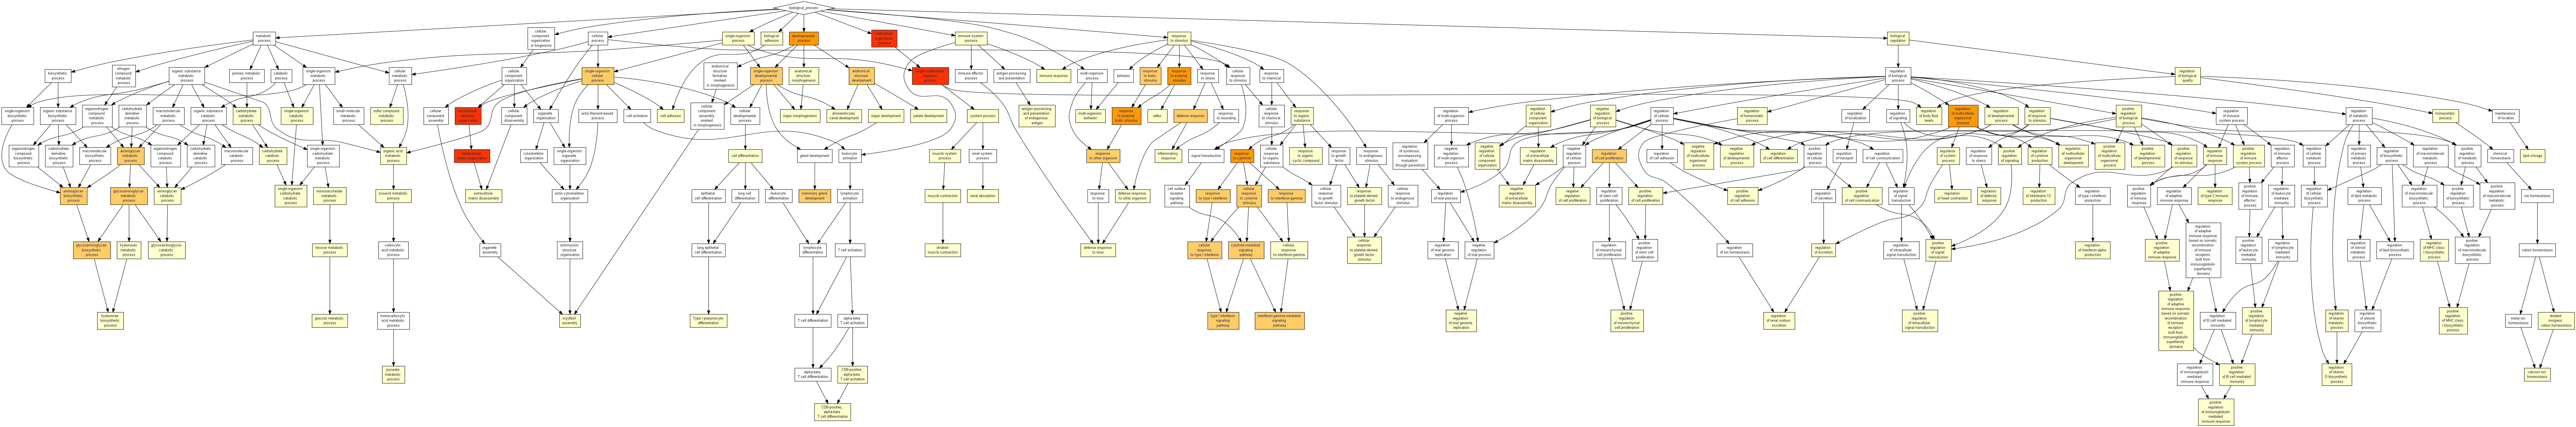
\includegraphics[width=\textwidth]
{Figures/tfc-go-all-graph/tfc-go-all-graph.png}
\caption{Vue d'ensemble}
\end{subfigure}
\end{sidewaysfigure}

\begin{figure}[p]
\ContinuedFloat
\begin{subfigure}{\textwidth}
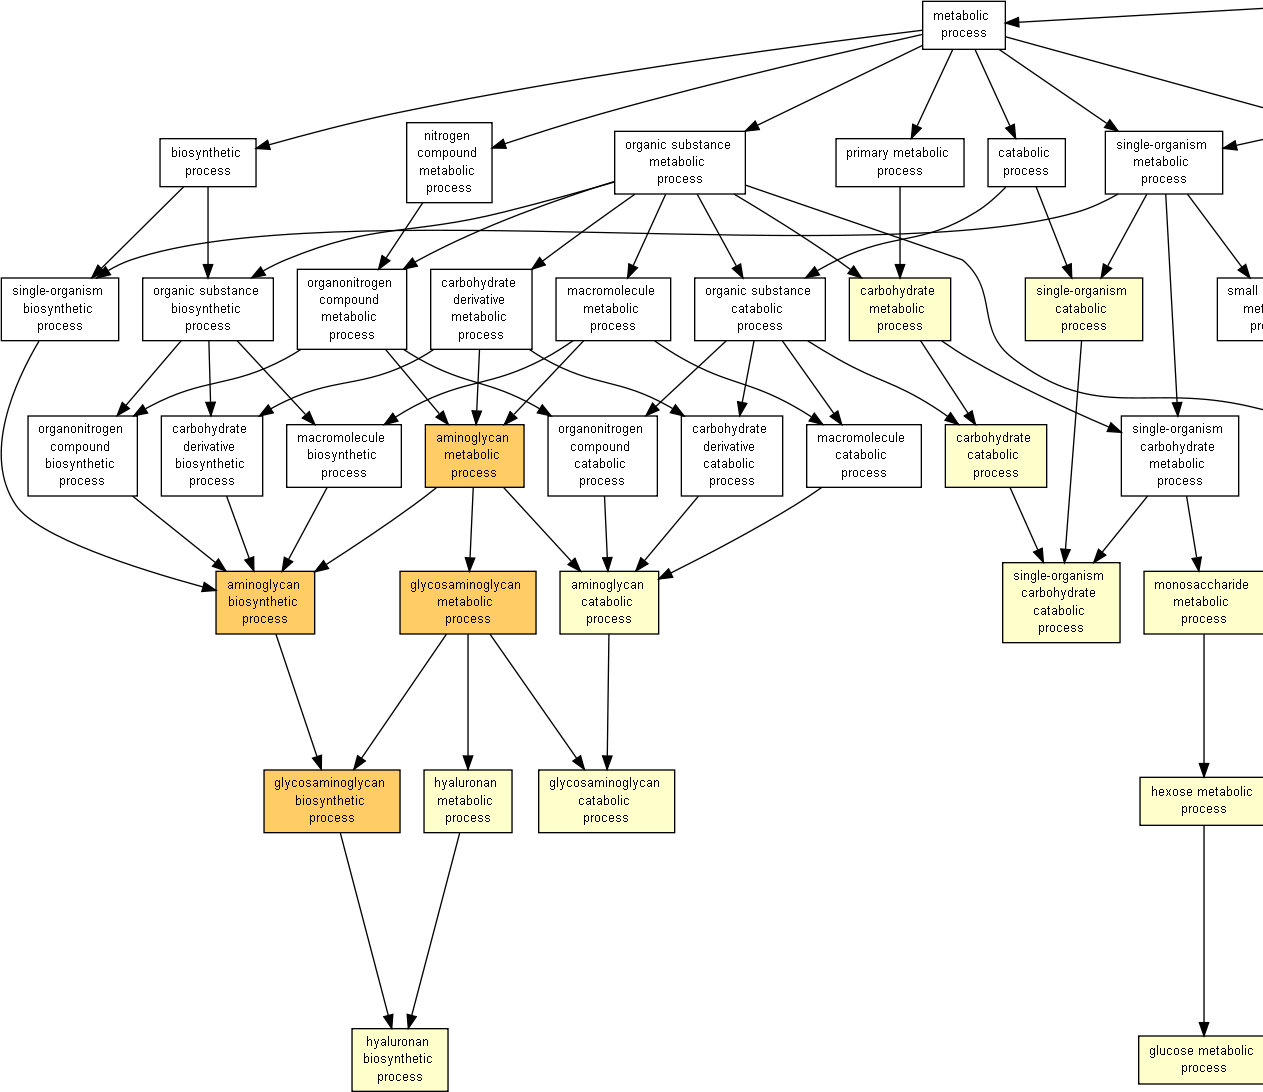
\includegraphics[width=\textwidth]
{Figures/tfc-go-all-graph/tfc-go-all-graph_0.png}
\caption{1/8}
\end{subfigure}
\end{figure}

\begin{figure}[p]
\ContinuedFloat
\begin{subfigure}{\textwidth}
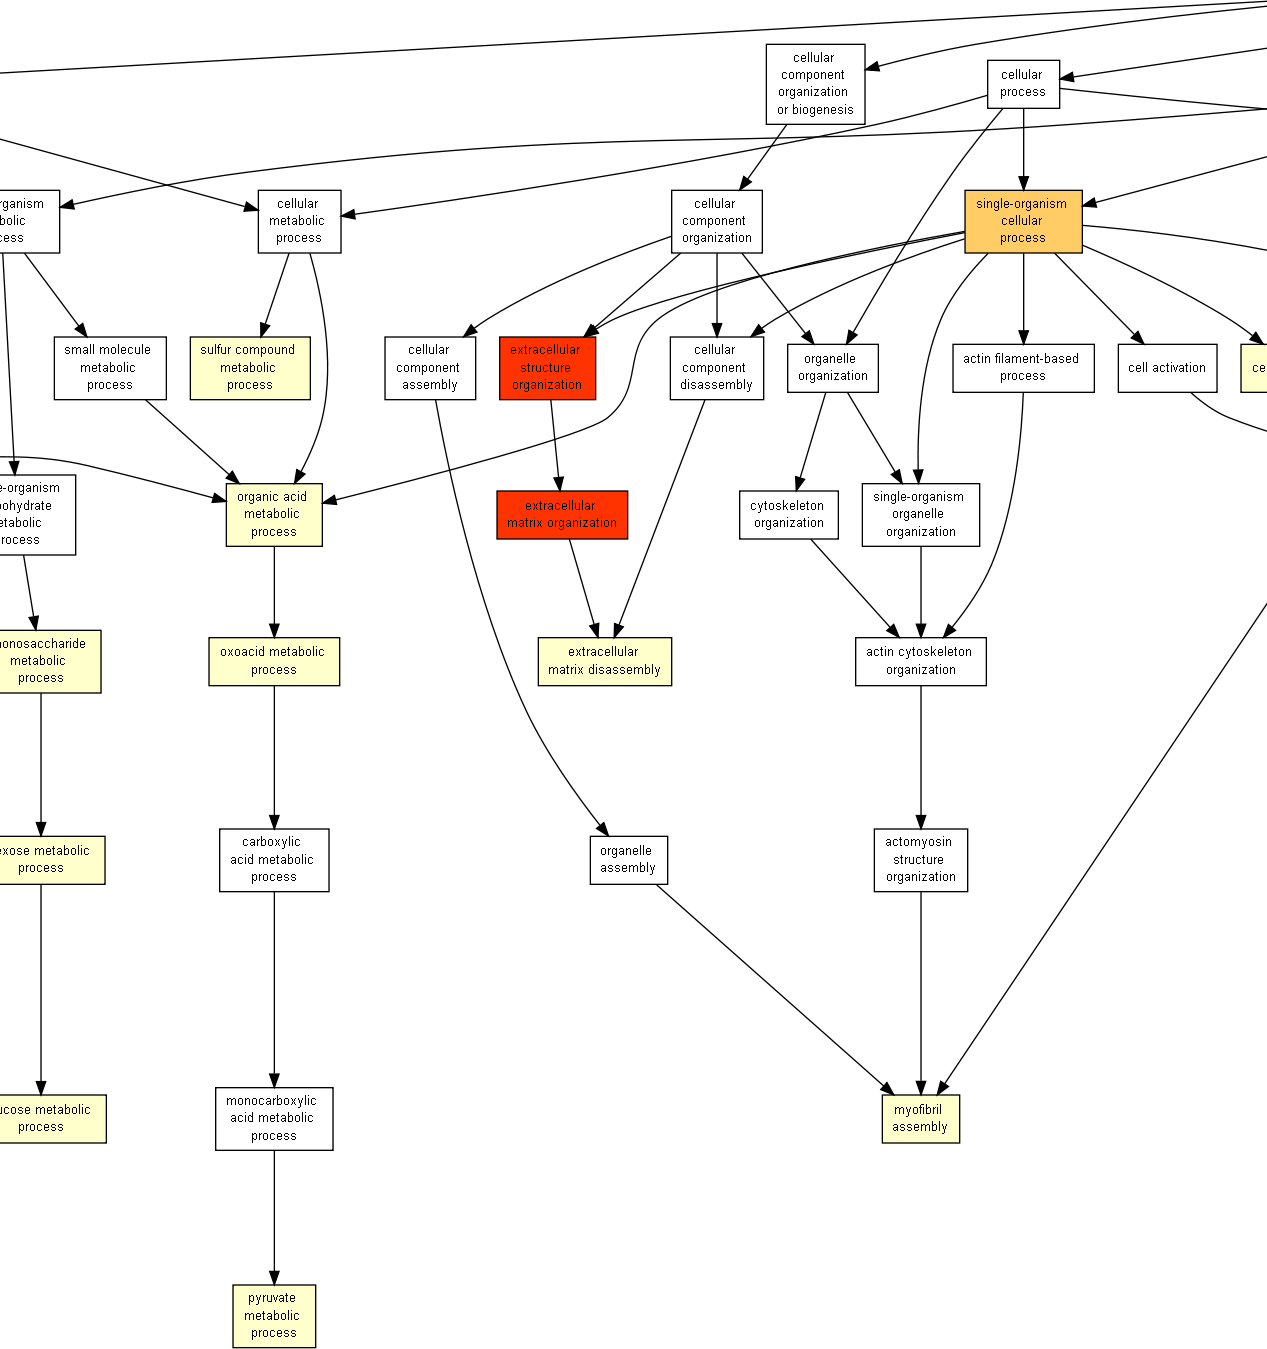
\includegraphics[width=\textwidth]
{Figures/tfc-go-all-graph/tfc-go-all-graph_1.png}
\caption{2/8}
\end{subfigure}
\end{figure}

\begin{figure}[p]
\ContinuedFloat
\begin{subfigure}{\textwidth}
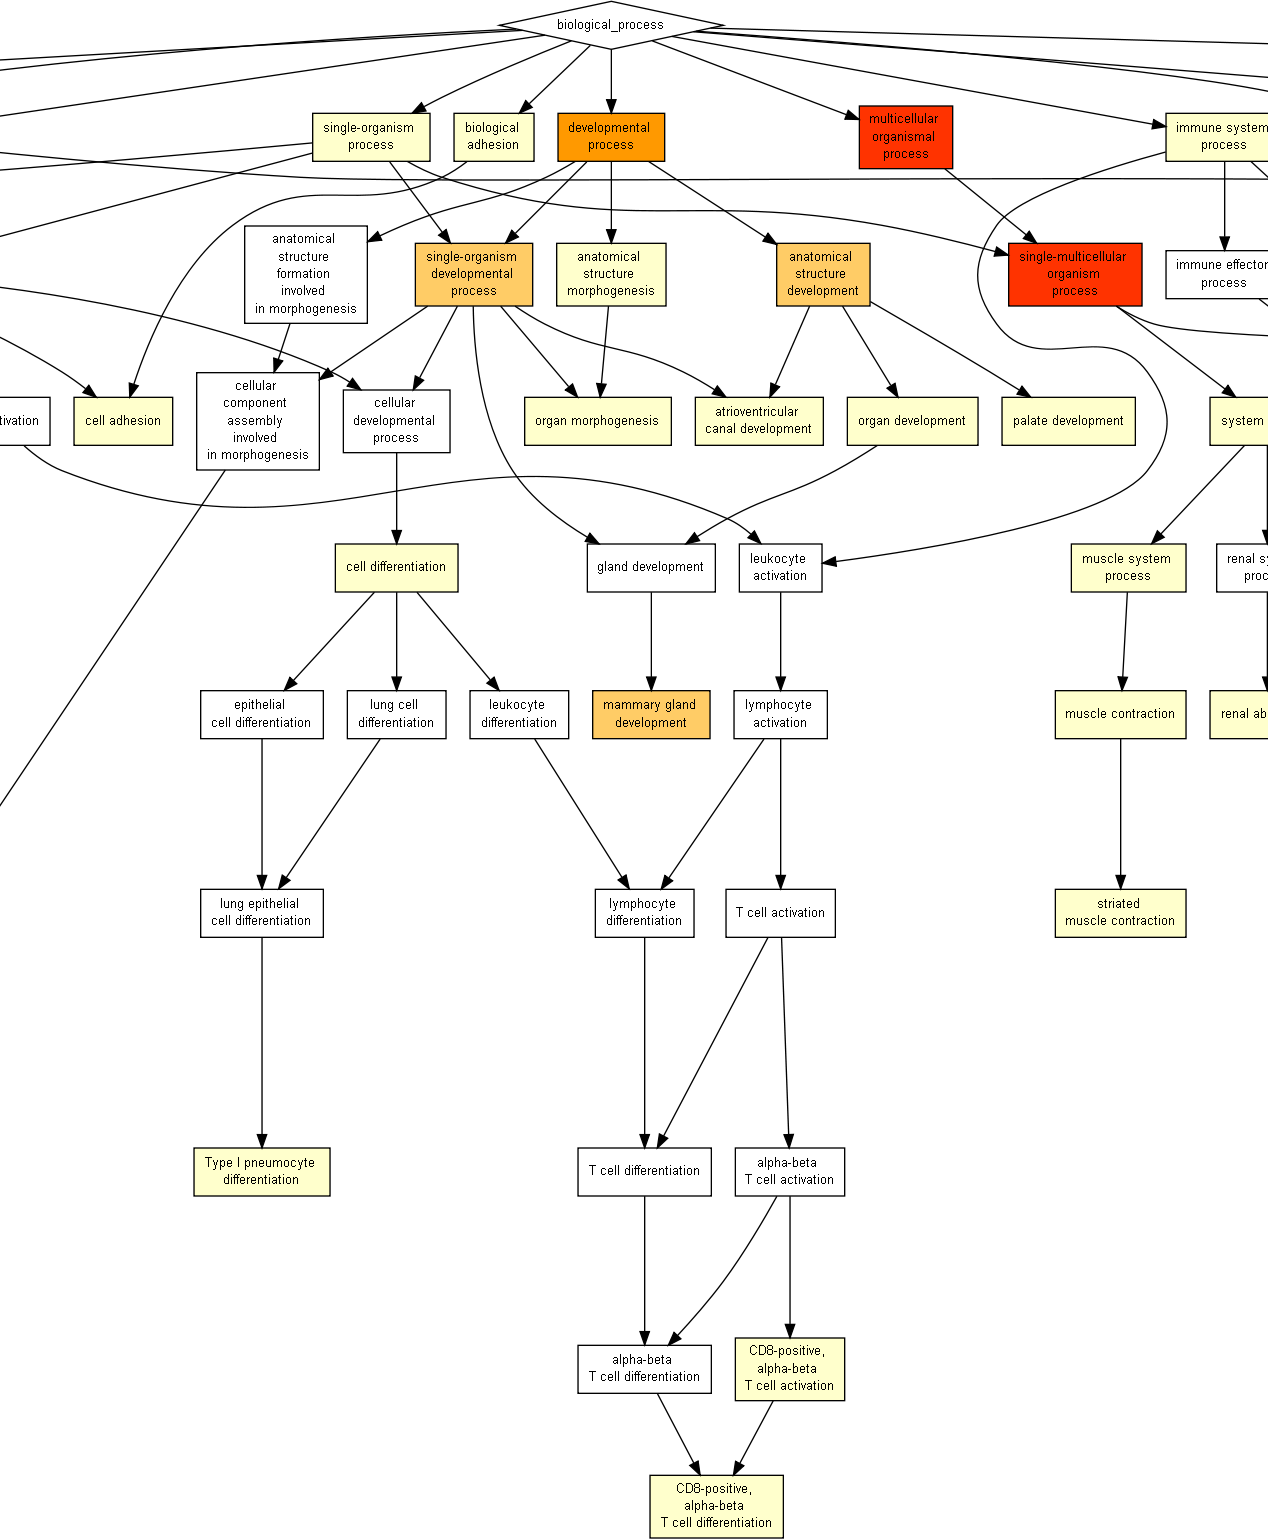
\includegraphics[width=\textwidth]
{Figures/tfc-go-all-graph/tfc-go-all-graph_2.png}
\caption{3/8}
\end{subfigure}
\end{figure}

\begin{figure}[p]
\ContinuedFloat
\begin{subfigure}{\textwidth}
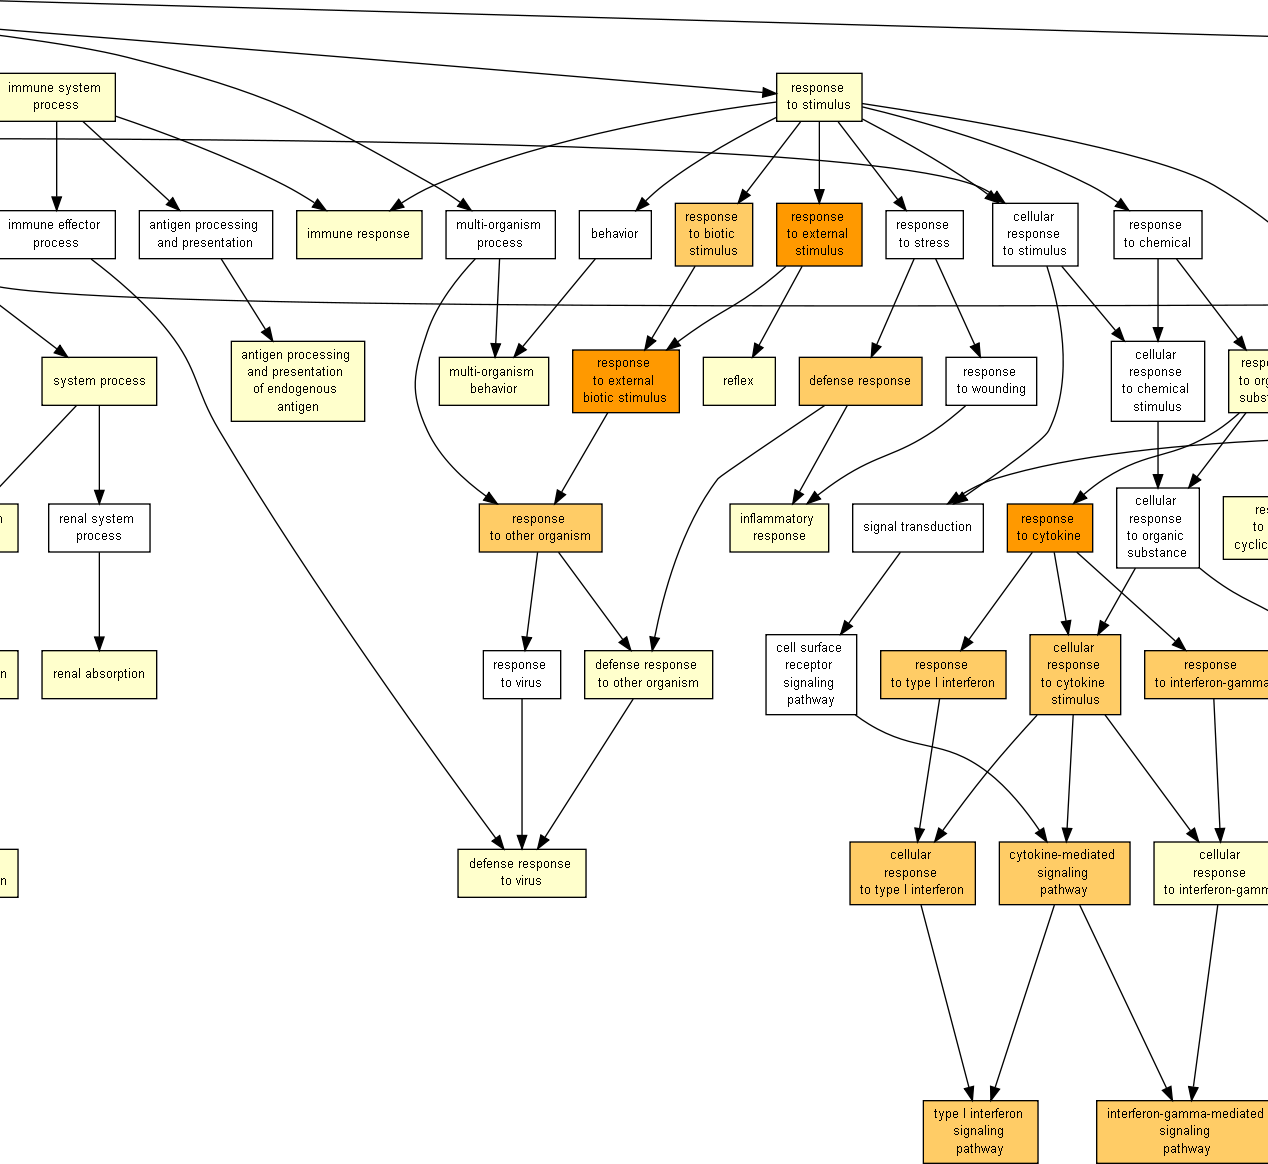
\includegraphics[width=\textwidth]
{Figures/tfc-go-all-graph/tfc-go-all-graph_3.png}
\caption{4/8}
\end{subfigure}
\end{figure}

\begin{figure}[p]
\ContinuedFloat
\begin{subfigure}{\textwidth}
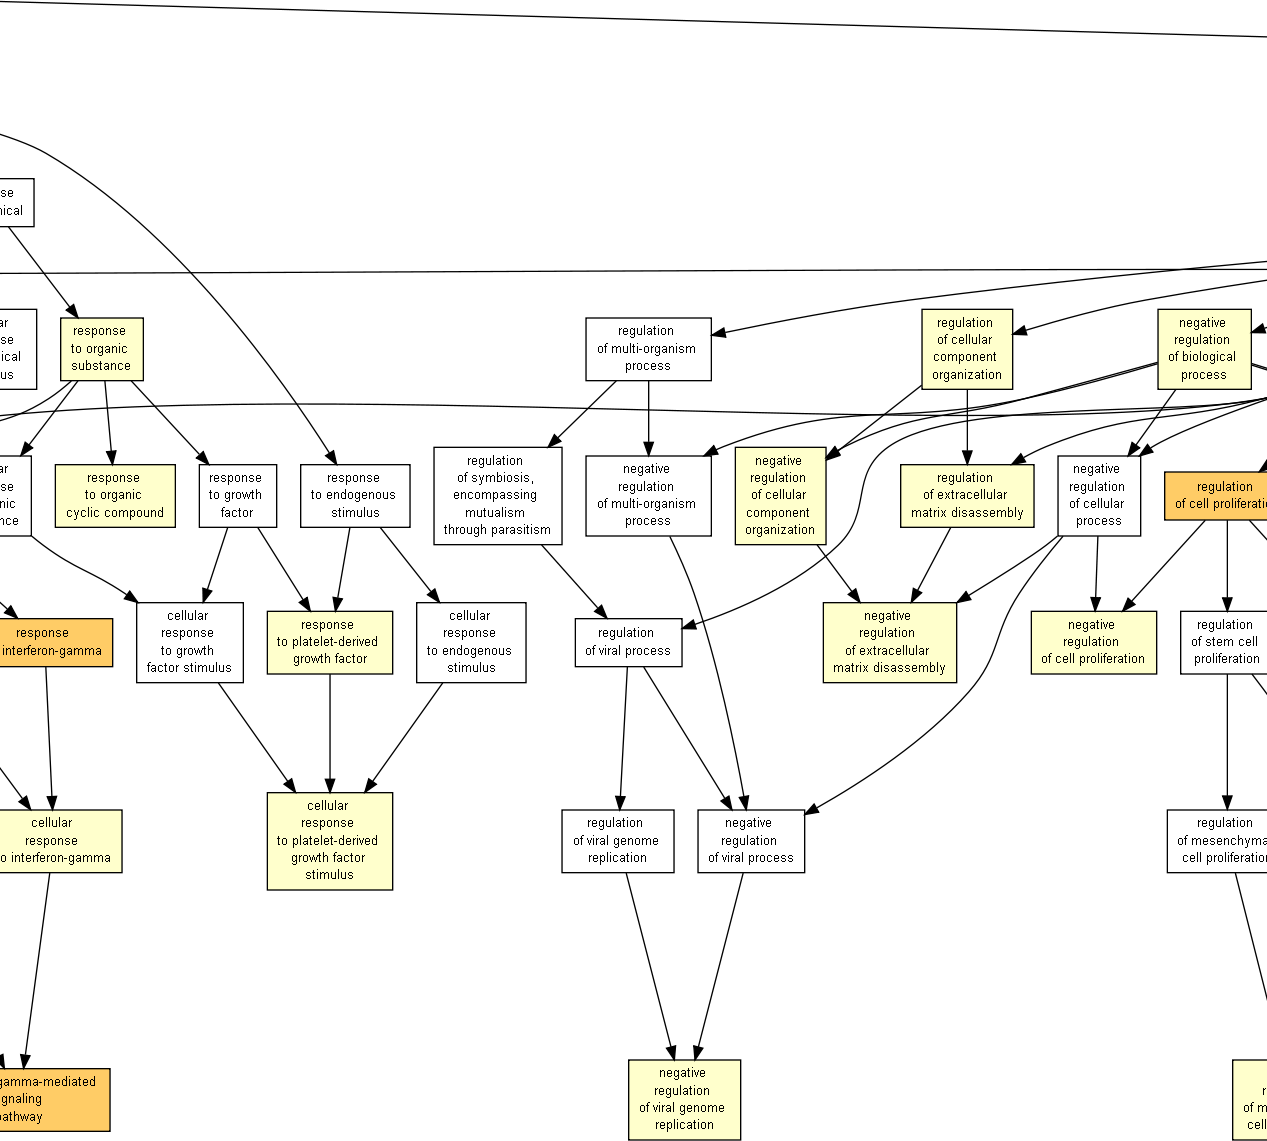
\includegraphics[width=\textwidth]
{Figures/tfc-go-all-graph/tfc-go-all-graph_4.png}
\caption{5/8}
\end{subfigure}
\end{figure}

\begin{figure}[p]
\ContinuedFloat
\begin{subfigure}{\textwidth}
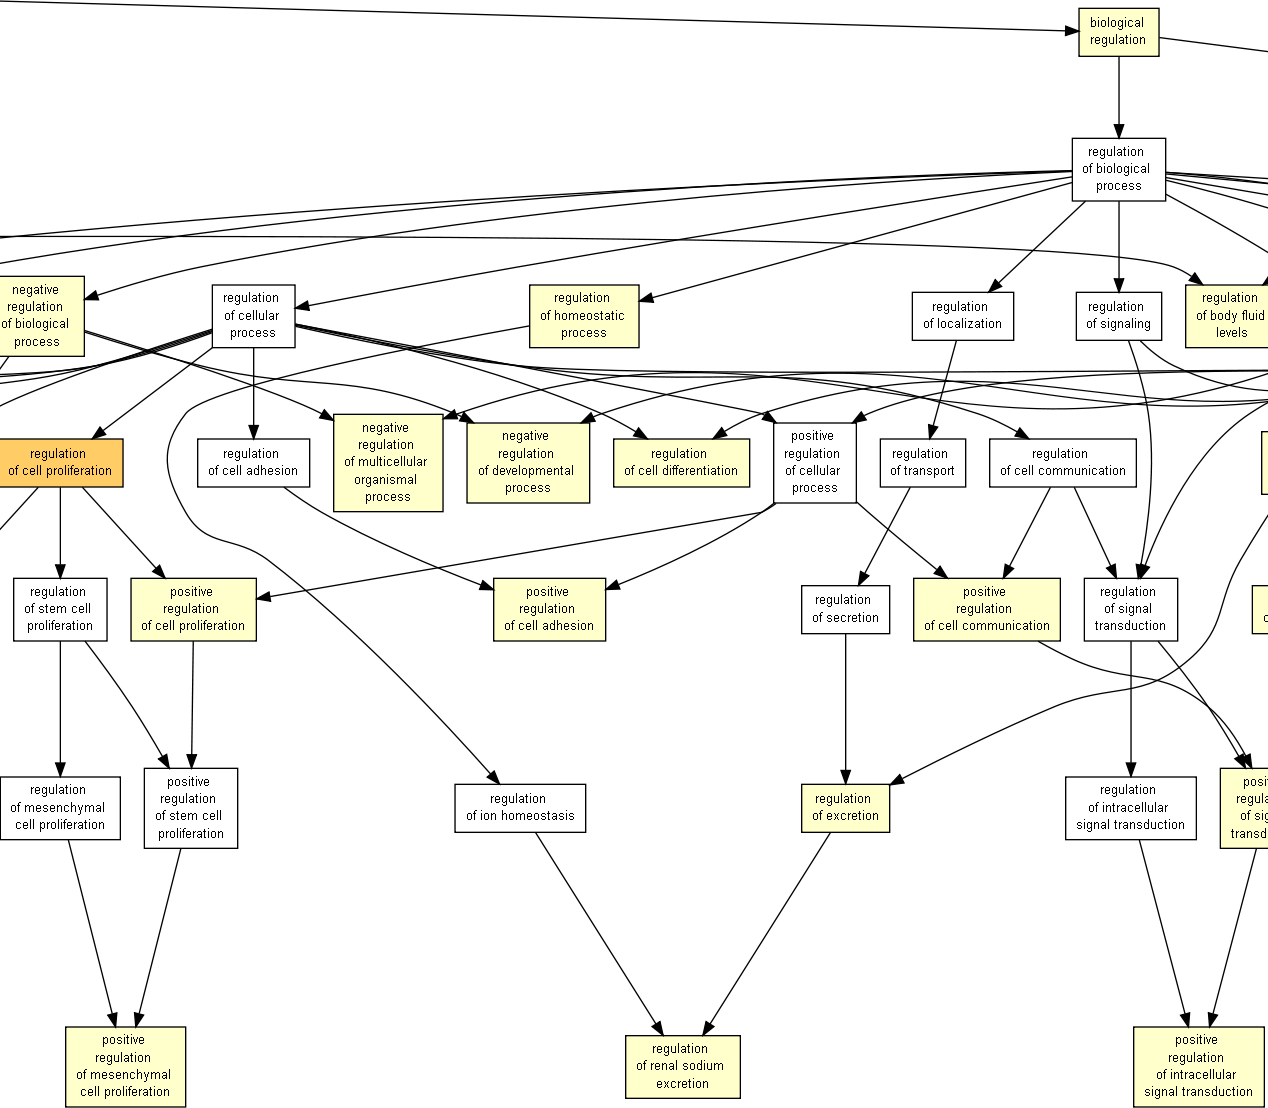
\includegraphics[width=\textwidth]
{Figures/tfc-go-all-graph/tfc-go-all-graph_5.png}
\caption{6/8}
\end{subfigure}
\end{figure}

\begin{figure}[p]
\ContinuedFloat
\begin{subfigure}{\textwidth}
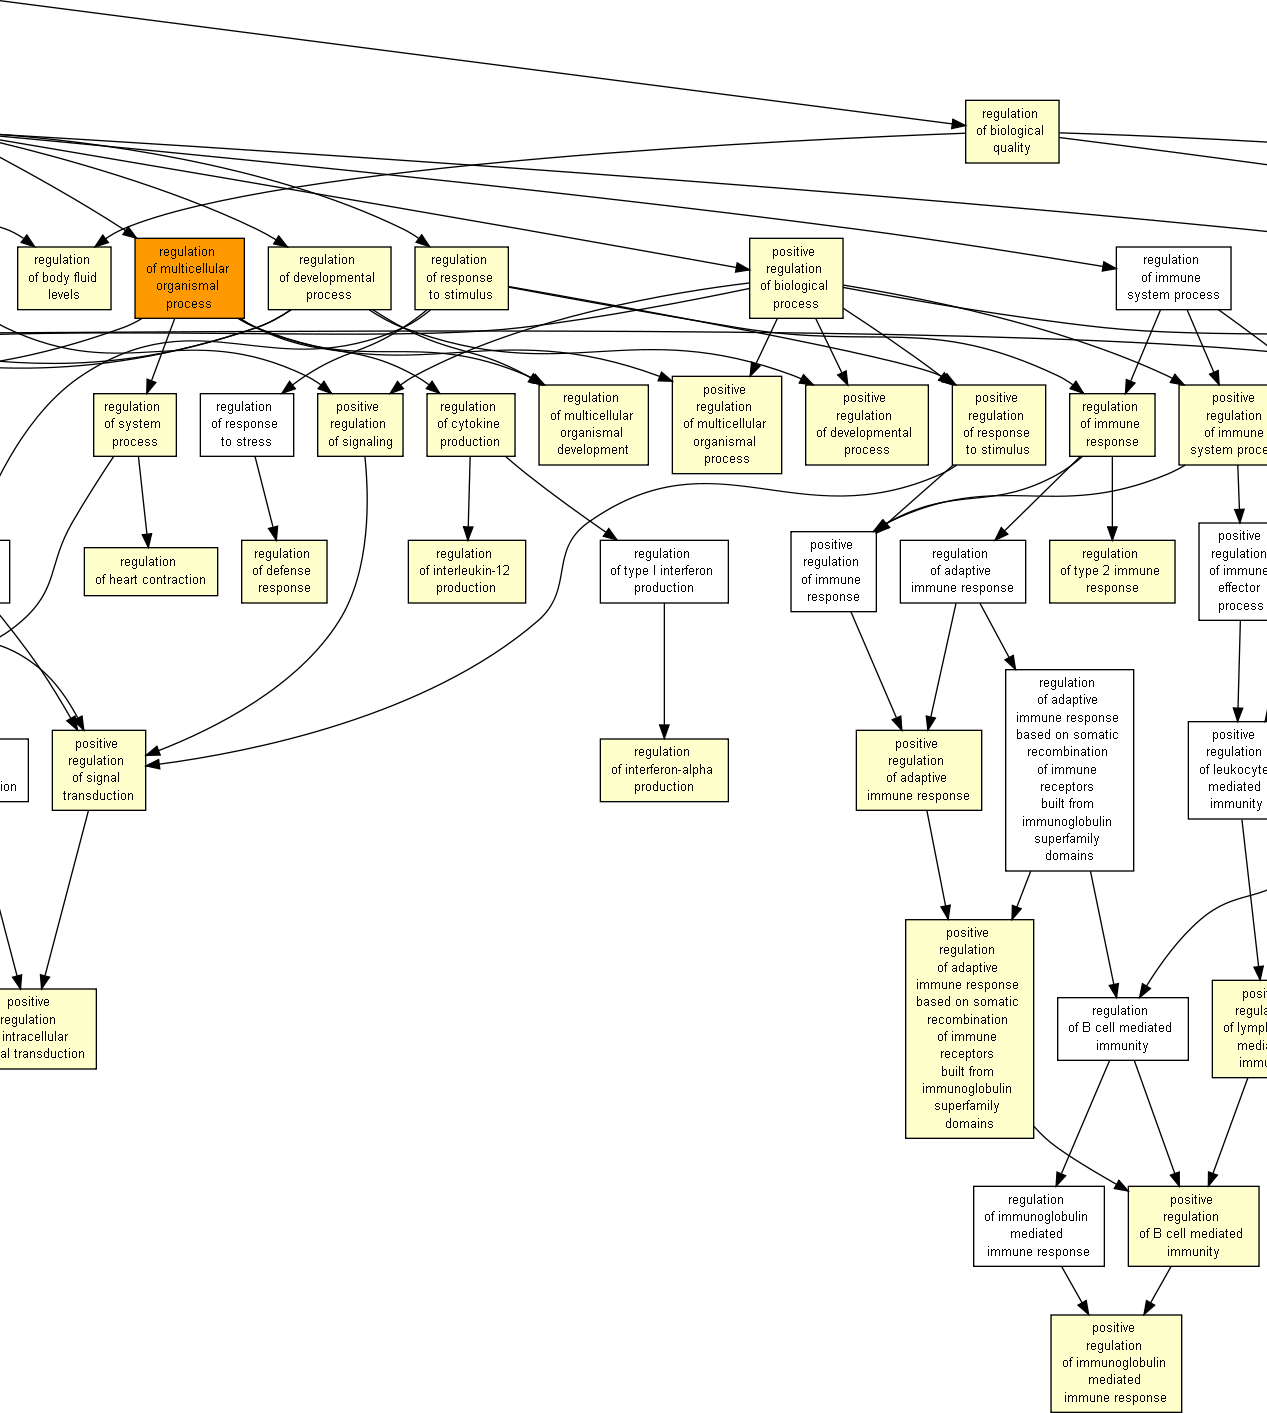
\includegraphics[width=\textwidth]
{Figures/tfc-go-all-graph/tfc-go-all-graph_6.png}
\caption{7/8}
\end{subfigure}
\end{figure}

\begin{figure}[!htp]
\ContinuedFloat
\begin{subfigure}{\textwidth}
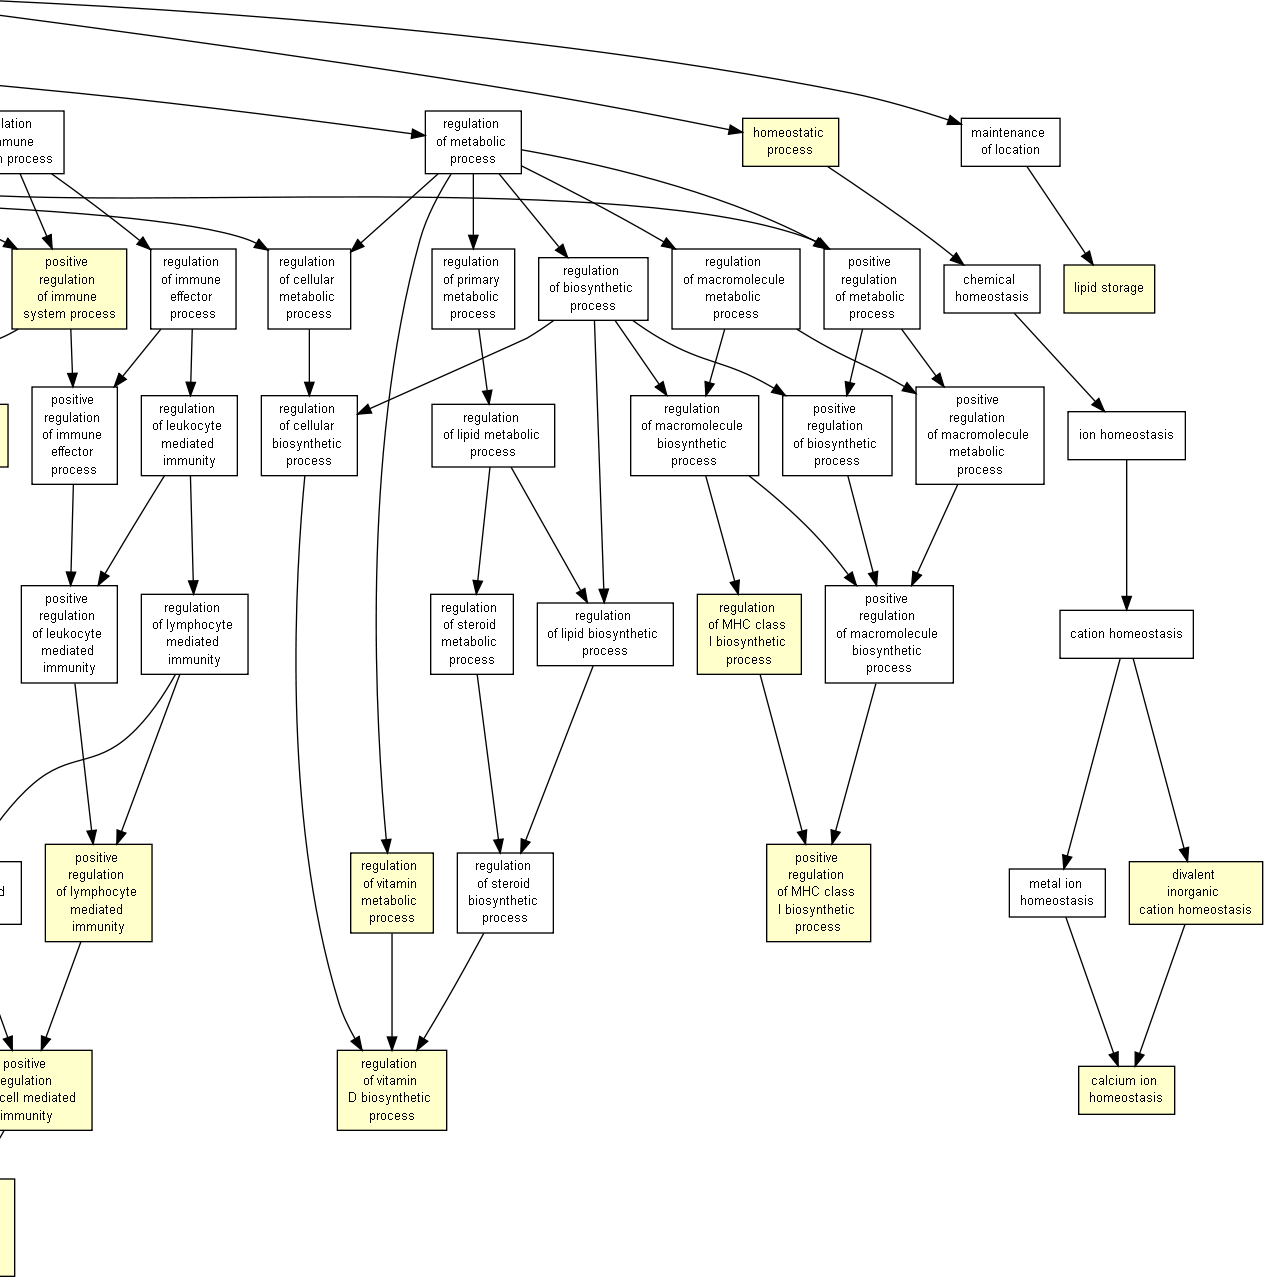
\includegraphics[width=\textwidth]
{Figures/tfc-go-all-graph/tfc-go-all-graph_7.png}
\caption{8/8}
\end{subfigure}
\caption[Enrichissement des catégories fonctionnelles associées aux gènes différentiellement exprimés dans l'épiderme caudal]
{
(Neuf pages précédentes) Enrichissement des catégories fonctionnelles associées aux gènes différentiellement exprimés dans l'épiderme caudal.
a) Vue d'ensemble.
b-i) Détail.
L'enrichissement des termes comparé à l'ensemble des gènes transcrits est calculé à l'aide de GOrilla \citep{Eden2009}.
Les couleurs des boites correspondent à la significativité de l'enrichissement.
Jaune pâle : $10^{-5} \leq p < 10^{-3}$
Jaune : $10^{-7} \leq p < 10^{-5}$
Orange : $10^{-9} \leq p < 10^{-7}$
Rouge: $p < 10^{-9}$
}
\label{fig:tfc-go-all-graph}
\end{figure}

La représentation en "treemap" décrite précédemment récapitule les fonctions biologiques enrichies (\autoref{fig:tfc-go-all-treemap}).

\begin{sidewaysfigure}[!htbp]
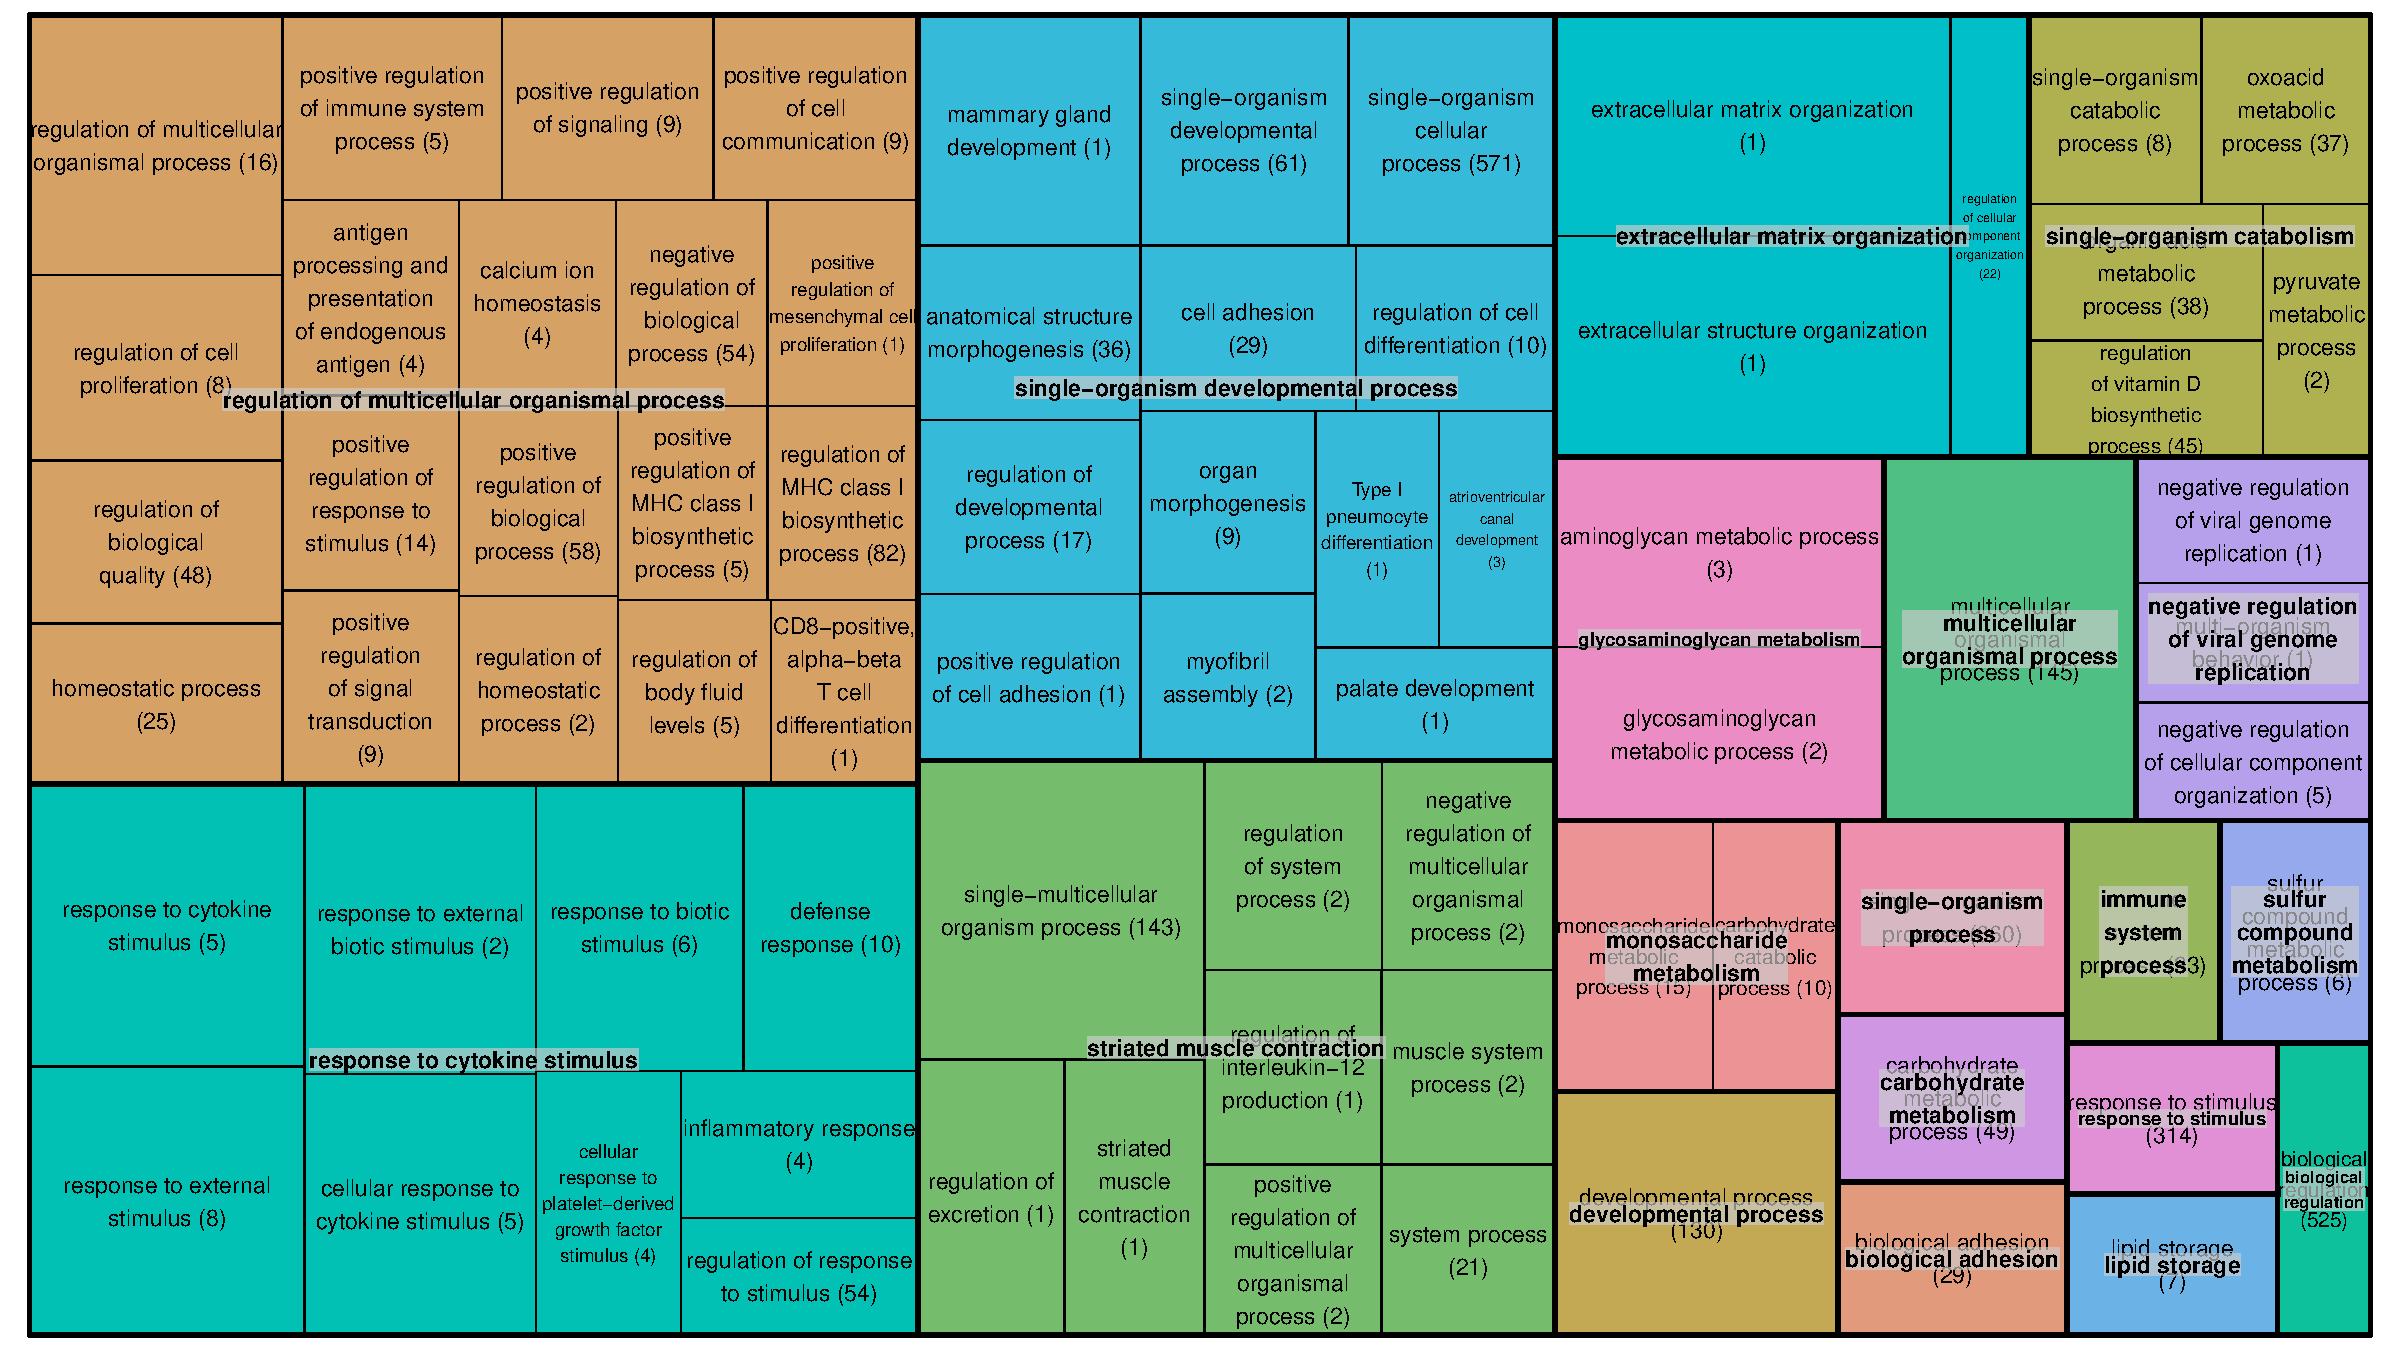
\includegraphics[width=\textwidth]
{Figures/tfc-go-all-treemap/tfc-go-all-treemap.pdf}
\caption[Enrichissement des catégories fonctionnelles associées aux gènes différentiellement exprimés dans l'épiderme caudal]
{
Enrichissement des catégories fonctionnelles associées aux gènes différentiellement exprimés dans l'épiderme caudal.
L'enrichissement de catégories fonctionnelles a été calculé à l'aide de GOrilla \citep{Eden2009}.
Les termes ont ensuite subit un post traitement à l'aide de REViGO \citep{Supek2011} afin de les représenter sous forme de "treemap".
La taille des rectangles est proportionnelle à la significativité de l'enrichissement de la catégorie fonctionnelle associée.
}
\label{fig:tfc-go-all-treemap}
\end{sidewaysfigure}

Au vu des données générées, les interactions entre signalisation \gls{ht} et \gls{gc} au niveau transcriptionnel se caractérisent, de façon similaire aux \glspl{hlb}, par deux types de profils :
\begin{itemize}
\item des profils type "potentialisation", où le traitement combiné des deux hormones se traduit par un effet plus marqué sur la quantité de transcrits des gènes cible que lors d'un traitement par une des deux hormones seule.
\item des profils de type "antagonisme", où l'effet d'une hormone est inhibé par la seconde.
\end{itemize}

Peu de gènes présentent un profil d'expression "antagonisé" par rapport à un profil d'expression de type "potentié", 129 et 747 respectivement.
Les profils de type "potentiés" peuvent être catégorisés en une potentiation de l'effet répresseur (\autoref{fig:tfc-clusters-pot}~A) et de l'effet activateur (\autoref{fig:tfc-clusters-pot}~B).
Les effets de type antagonistes sont marqués par la présence de "clusters" regroupant des gènes dont l'effet de la \gls{t3} est inhibé par la \gls{cort} (\autoref{fig:tfc-clusters-antago}~A) et des gènes dont l'effet de la \gls{cort} est inhibé par celui de la \gls{t3} (\autoref{fig:tfc-clusters-antago}~B).

% BOTTOM caption
% ------------------------
\begin{figure}[!htbp]
\centering
\vspace{1\baselineskip}
\includegraphics[width=\textwidth]
% ------------------------
%
% SIDE caption
% ------------------------
%\begin{SCfigure}[\sidecaptionrelwidth][!htbp]
%\centering
%\vspace{1\baselineskip}
%\includegraphics[width=0.5\textwidth]
% ------------------------
%
% Main information
% ===========================================================
{Figures/tfc-clusters-pot/tfc-clusters-pot.pdf}
\caption[Partitionnement des profils d'expression des gènes de type ``potentiation'']
{
Partitionnement des profils d'expression des gènes de type ``potentiation''.
La variance des niveaux d'expression à travers les quatres traitements est normalisée à 1 et la moyenne centrée sur 0.
A) Gènes réprimés.
B) Gènes induits.
$\emptyset$ : Contrôle; T : \gls{t3}; C : \gls{cort}; CT : \gls{cort} + \gls{t3}
}
\label{fig:tfc-clusters-pot}
% ===========================================================
%
% BOTTOM caption
% ------------------------
\end{figure}
% ------------------------
%
% SIDE caption
% ------------------------
%\end{SCfigure}
% ------------------------
%
%
%\missingfigure{Clusters effet potentiateur}

% BOTTOM caption
% ------------------------
\begin{figure}[!htbp]
\centering
\vspace{1\baselineskip}
\includegraphics[width=\textwidth]
% ------------------------
%
% SIDE caption
% ------------------------
%\begin{SCfigure}[\sidecaptionrelwidth][!htbp]
%\centering
%\vspace{1\baselineskip}
%\includegraphics[width=0.5\textwidth]
% ------------------------
%
% Main information
% ===========================================================
{Figures/tfc-clusters-antago/tfc-clusters-antago.pdf}
\caption[Partitionnement des profils d'expression des gènes de type ``antagonisme'']
{Partitionnement des profils d'expression des gènes types ``antagonisme''.
La variance des niveaux d'expression à travers les quatres traitements est normalisée à 1 et la moyenne centrée sur 0.
A) Inhibition de l'effet \gls{t3} par la \gls{cort}.
B) Inhibition de l'effet \gls{cort} par la \gls{t3}.
$\emptyset$ : Contrôle; T : \gls{t3}; C : \gls{cort}; CT : \gls{cort} + \gls{t3}
}
\label{fig:tfc-clusters-antago}
% ===========================================================
%
% BOTTOM caption
% ------------------------
\end{figure}
% ------------------------
%
% SIDE caption
% ------------------------
%\end{SCfigure}
% ------------------------
%
%
%\missingfigure{Clusters effets antagoniste}

Pour mettre en évidence les catégories fonctionnelles spécifiques des diférents types d'interactions croisées entre \glspl{ht} et \glspl{gc}, le "background" que j'ai utilisé a été constitué à partir de la liste des 1363 gènes différentiellement exprimés dans au moins une condition.
Les fonctions biologiques associées aux gènes réprimés parmi les gènes "potentialisés" sont clairement associées à l'inhibition de prolifération cellulaire et à la réponse immunitaire  \autoref{fig:tfc-go-pot-down}.

% BOTTOM caption
% ------------------------
\begin{figure}[!htbp]
\centering
\vspace{1\baselineskip}
\includegraphics[width=\textwidth]
% ------------------------
%
% SIDE caption
% ------------------------
%\begin{SCfigure}[\sidecaptionrelwidth][!htbp]
%\centering
%\vspace{1\baselineskip}
%\includegraphics[width=0.5\textwidth]
% ------------------------
%
% Main information
% ===========================================================
{Figures/tfc-go-pot-down/tfc-go-pot-down.png}
\caption[Catégories fonctionnelles enrichies parmi les gènes réprimés de type ``potentiation'']
{
Catégories fonctionnelles enrichies parmi les gènes réprimés ``potentiation'', correspondants aux clusters 1, 2, 3 et 4 de la \autoref{fig:tfc-clusters-pot}~A.
Les catégories fonctionnelles enrichies ont été obtenues à l'aide de GOrilla \citep{Eden2009}.
Les couleurs des boites correspondent à la significativité de l'enrichissement.
Jaune pâle : $10^{-5} \leq p < 10^{-3}$.
Orange : $10^{-7} \leq p < 10^{-5}$.
}
\label{fig:tfc-go-pot-down}
% ===========================================================
%
% BOTTOM caption
% ------------------------
\end{figure}
% ------------------------
%
% SIDE caption
% ------------------------
%\end{SCfigure}
% ------------------------
%
%
%\missingfigure{Make a figure}

Les gènes dont la quantité de transcrits est augmentée de façon potentiée par le traitement combiné des deux hormones sont caractéristiques de fonctions biologiques liés au transport d'ions organiques et de molécules de petite taille. \autoref{fig:tfc-go-pot-up}.

% BOTTOM caption
% ------------------------
%\begin{figure}[!htbp]
%\centering
%\vspace{1\baselineskip}
%\includegraphics[width=\textwidth]
% ------------------------
%
% SIDE caption
% ------------------------
\begin{SCfigure}[\sidecaptionrelwidth][!htbp]
\centering
\vspace{1\baselineskip}
\includegraphics[width=0.5\textwidth]
% ------------------------
%
% Main information
% ===========================================================
{Figures/tfc-go-pot-up/tfc-go-pot-up.png}
\caption[Catégories fonctionnelles enrichies parmi les gènes induits "potentiés"]
{
Catégories fonctionnelles enrichies parmi les gènes induits "potentiés", correspondants aux clusters 5, 6 et 7 de la \autoref{fig:tfc-clusters-pot}~B.
Les catégories fonctionnelles enrichies ont été obtenues à l'aide de GOrilla \citep{Eden2009}.
Les couleurs des boites correspondent à la significativité de l'enrichissement.
Jaune pâle : $10^{-3} \leq p < 10^{-5}$
}
\label{fig:tfc-go-pot-up}
% ===========================================================
%
% BOTTOM caption
% ------------------------
%\end{figure}
% ------------------------
%
% SIDE caption
% ------------------------
\end{SCfigure}
% ------------------------
%
%
%\missingfigure{Make a figure}

Les "clusters" regroupant les gènes dont les effets des \glspl{ht} et des \glspl{gc} s'antagonisent ne présentent pas d'enrichissement particulièrement fort pour une ou plusieurs fonctions biologiques définies.
Il semble toutefois que les le transport membranaire d'ions soit légèrement sur-représenté dans ces catégories (\autoref{fig:tfc-go-antago-cort} et \autoref{fig:tfc-go-antago-t3}).

% BOTTOM caption
% ------------------------
\begin{figure}[!htbp]
\centering
\vspace{1\baselineskip}
\includegraphics[width=\textwidth]
% ------------------------
%
% SIDE caption
% ------------------------
%\begin{SCfigure}[\sidecaptionrelwidth][!htbp]
%\centering
%\vspace{1\baselineskip}
%\includegraphics[width=0.5\textwidth]
% ------------------------
%
% Main information
% ===========================================================
{Figures/tfc-go-antago-cort/tfc-go-antago-cort.pdf}
\caption[Catégories fonctionnelles enrichies parmi les gènes présentant une inhibition de l'effet \gls{cort} par la \gls{t3}]
{
Catégories fonctionnelles enrichies parmi les gènes présentant une inhibition de l'effet \gls{cort} par la \gls{t3}, correspondants aux clusters 5 et 6 de la \autoref{fig:tfc-clusters-antago}~B.
A) Gènes réprimés par la \gls{cort} (cluster 5, \autoref{fig:tfc-clusters-antago}~B).
B) Gènes induits par la \gls{cort} (cluster 6, \autoref{fig:tfc-clusters-antago}~B).
Les catégories fonctionnelles enrichies ont été obtenues à l'aide de GOrilla \citep{Eden2009}.
Les couleurs des boites correspondent à la significativité de l'enrichissement.
Jaune pâle : $10^{-5} \leq p < 10^{-3}$
Orange : $10^{-7} \leq p < 10^{-5}$
}
\label{fig:tfc-go-antago-cort}
% ===========================================================
%
% BOTTOM caption
% ------------------------
\end{figure}
% ------------------------
%
% SIDE caption
% ------------------------
%\end{SCfigure}
% ------------------------
%
%
%\missingfigure{Make a figure}

% BOTTOM caption
% ------------------------
\begin{figure}[!htbp]
\centering
\vspace{1\baselineskip}
\includegraphics[width=0.3\textwidth]
% ------------------------
%
% SIDE caption
% ------------------------
%\begin{SCfigure}[\sidecaptionrelwidth][!htbp]
%\includegraphics[width=0.3\textwidth]
% ------------------------
%
% Main information
% ===========================================================
{Figures/tfc-go-antago-t3/tfc-go-antago-t3.png}
\caption[Catégories fonctionnelles enrichies parmi les gènes présentant une inhibition de l'effet \gls{t3} par la \gls{cort}]
{
Catégories fonctionnelles enrichies parmi les gènes présentant une inhibition de l'effet \gls{t3} par la \gls{cort}, correspondant au cluster 1 de la \autoref{fig:tfc-clusters-antago}~A.
Les clusters 2, 3 et 4 de la \autoref{fig:tfc-clusters-antago}~A ne présentent pas de catégories fonctionnelles enrichies.
Les catégories fonctionnelles enrichies ont été obtenues à l'aide de GOrilla \citep{Eden2009}.
Les couleurs des boites correspondent à la significativité de l'enrichissement.
Jaune pâle : $10^{-3} \leq p < 10^{-5}$
}
\label{fig:tfc-go-antago-t3}
% ===========================================================
%
% BOTTOM caption
% ------------------------
\end{figure}
% ------------------------
%
% SIDE caption
% ------------------------
%\end{SCfigure}
% ------------------------

Les gènes ayant des profils de type "antagonisé" et dans une moindre mesure de type "potentiés" ont des effets biologiques très divers, soulignant le caractère pléiotrope des \glspl{ht} et des \glspl{gc}.
Cette propriété, combinée à la taille restreinte des ensembles de gènes étudiés, contribue au faible enrichissement de catégories fonctionnelles par l'utilisation d'outils automatisés.


\section{Annotation fonctionnelle manuelle: complément à la caractérisation automatisée de termes enrichis}

Pour aller plus loin dans la caractérisation des effets biologiques de l'interaction entre les deux voies de signalisation, j'ai réalisé l'annotation fonctionnelle manuelle des gènes dans les différentes catégories de profil d'expression (voir \autoref{subsec:manual-annot}).

\subsection{Annotation manuelle des gènes régulés de façon croisée par les hormones thyroïdiennes et les glucocorticoïdes}
Les termes relevés et le nombre de gènes qui leur sont associés sont présentés \autoref{fig:tfc-manualannot-pot-vs-antago}.
Le contraste avec les méthodes d'annotation fonctionnelle automatisées est frappant:
L'annotation manuelle fait ressortir un nombre important de gènes associés au cytosquelette, à l'adhésion cellulaire, à la matrice extra-cellulaire, aux processus d'inflammation et de régulation de la prolifération cellulaire / apoptose.

% BOTTOM caption
% ------------------------
\begin{figure}[!htbp]
\centering
\vspace{1\baselineskip}
\includegraphics[width=0.9\textwidth]
% ------------------------
%
% SIDE caption
% ------------------------
%\begin{SCfigure}[\sidecaptionrelwidth][!htbp]
%\centering
%\vspace{1\baselineskip}
%\includegraphics[width=0.5\textwidth]
% ------------------------
%
% Main information
% ===========================================================
{Figures/tfc-manualannot-pot-vs-antago/tfc-manualannot-pot-vs-antago.png}
\caption[Termes enrichis dans les catégories de "potentiation" et d'"antagonisme" dans l'épiderme caudal]
{
Termes enrichis dans les catégories de gènes "antagonisés" (à gauches) et "potentiés" (à droite) dans l'épiderme caudal.
La valeur absolue de l'axe des abscisses représente le nombre de gène associé à chaque terme (axe des ordonnées).
Seuls les 50 termes les plus représenté sont illustrés ici.
Les barres verticales rouge correspondent au nombre théorique de gènes associés à chaque terme dans le cas d'une répartition aléatoire entre profils "antagonisés" et "potentiés".
}
\label{fig:tfc-manualannot-pot-vs-antago}
% ===========================================================
%
% BOTTOM caption
% ------------------------
\end{figure}
% ------------------------
%
% SIDE caption
% ------------------------
%\end{SCfigure}
% ------------------------

Enfin, il est intéressant de noter qu'il n'y a vraisemblablement pas de fonction biologique spécifiquement enrichie à chaque type interaction ("antagonisme" \textit{vs} "potentiation").


\subsection{Annotation manuelle des gènes constituant les profils "antagonisés"}
J'ai ensuite représenté séparément les termes associés aux gènes dont l'effet de la \gls{t3} est antagonisé par la \gls{cort} ("clusters" 1-4 \autoref{fig:tfc-clusters-antago}~A, \autoref{subfig:tfc-manualannot-antago-t}) et dont l'effet de la \gls{cort} est antagonisé par la \gls{t3} ("clusters" 5-6 \autoref{fig:tfc-clusters-antago}~B, \autoref{subfig:tfc-manualannot-antago-c}).

% BOTTOM caption
% ------------------------
\begin{figure}[!htbp]
\centering
\vspace{1\baselineskip}
% ------------------------
%
% Main information
% ===========================================================
\begin{subfigure}{0.49\textwidth}
	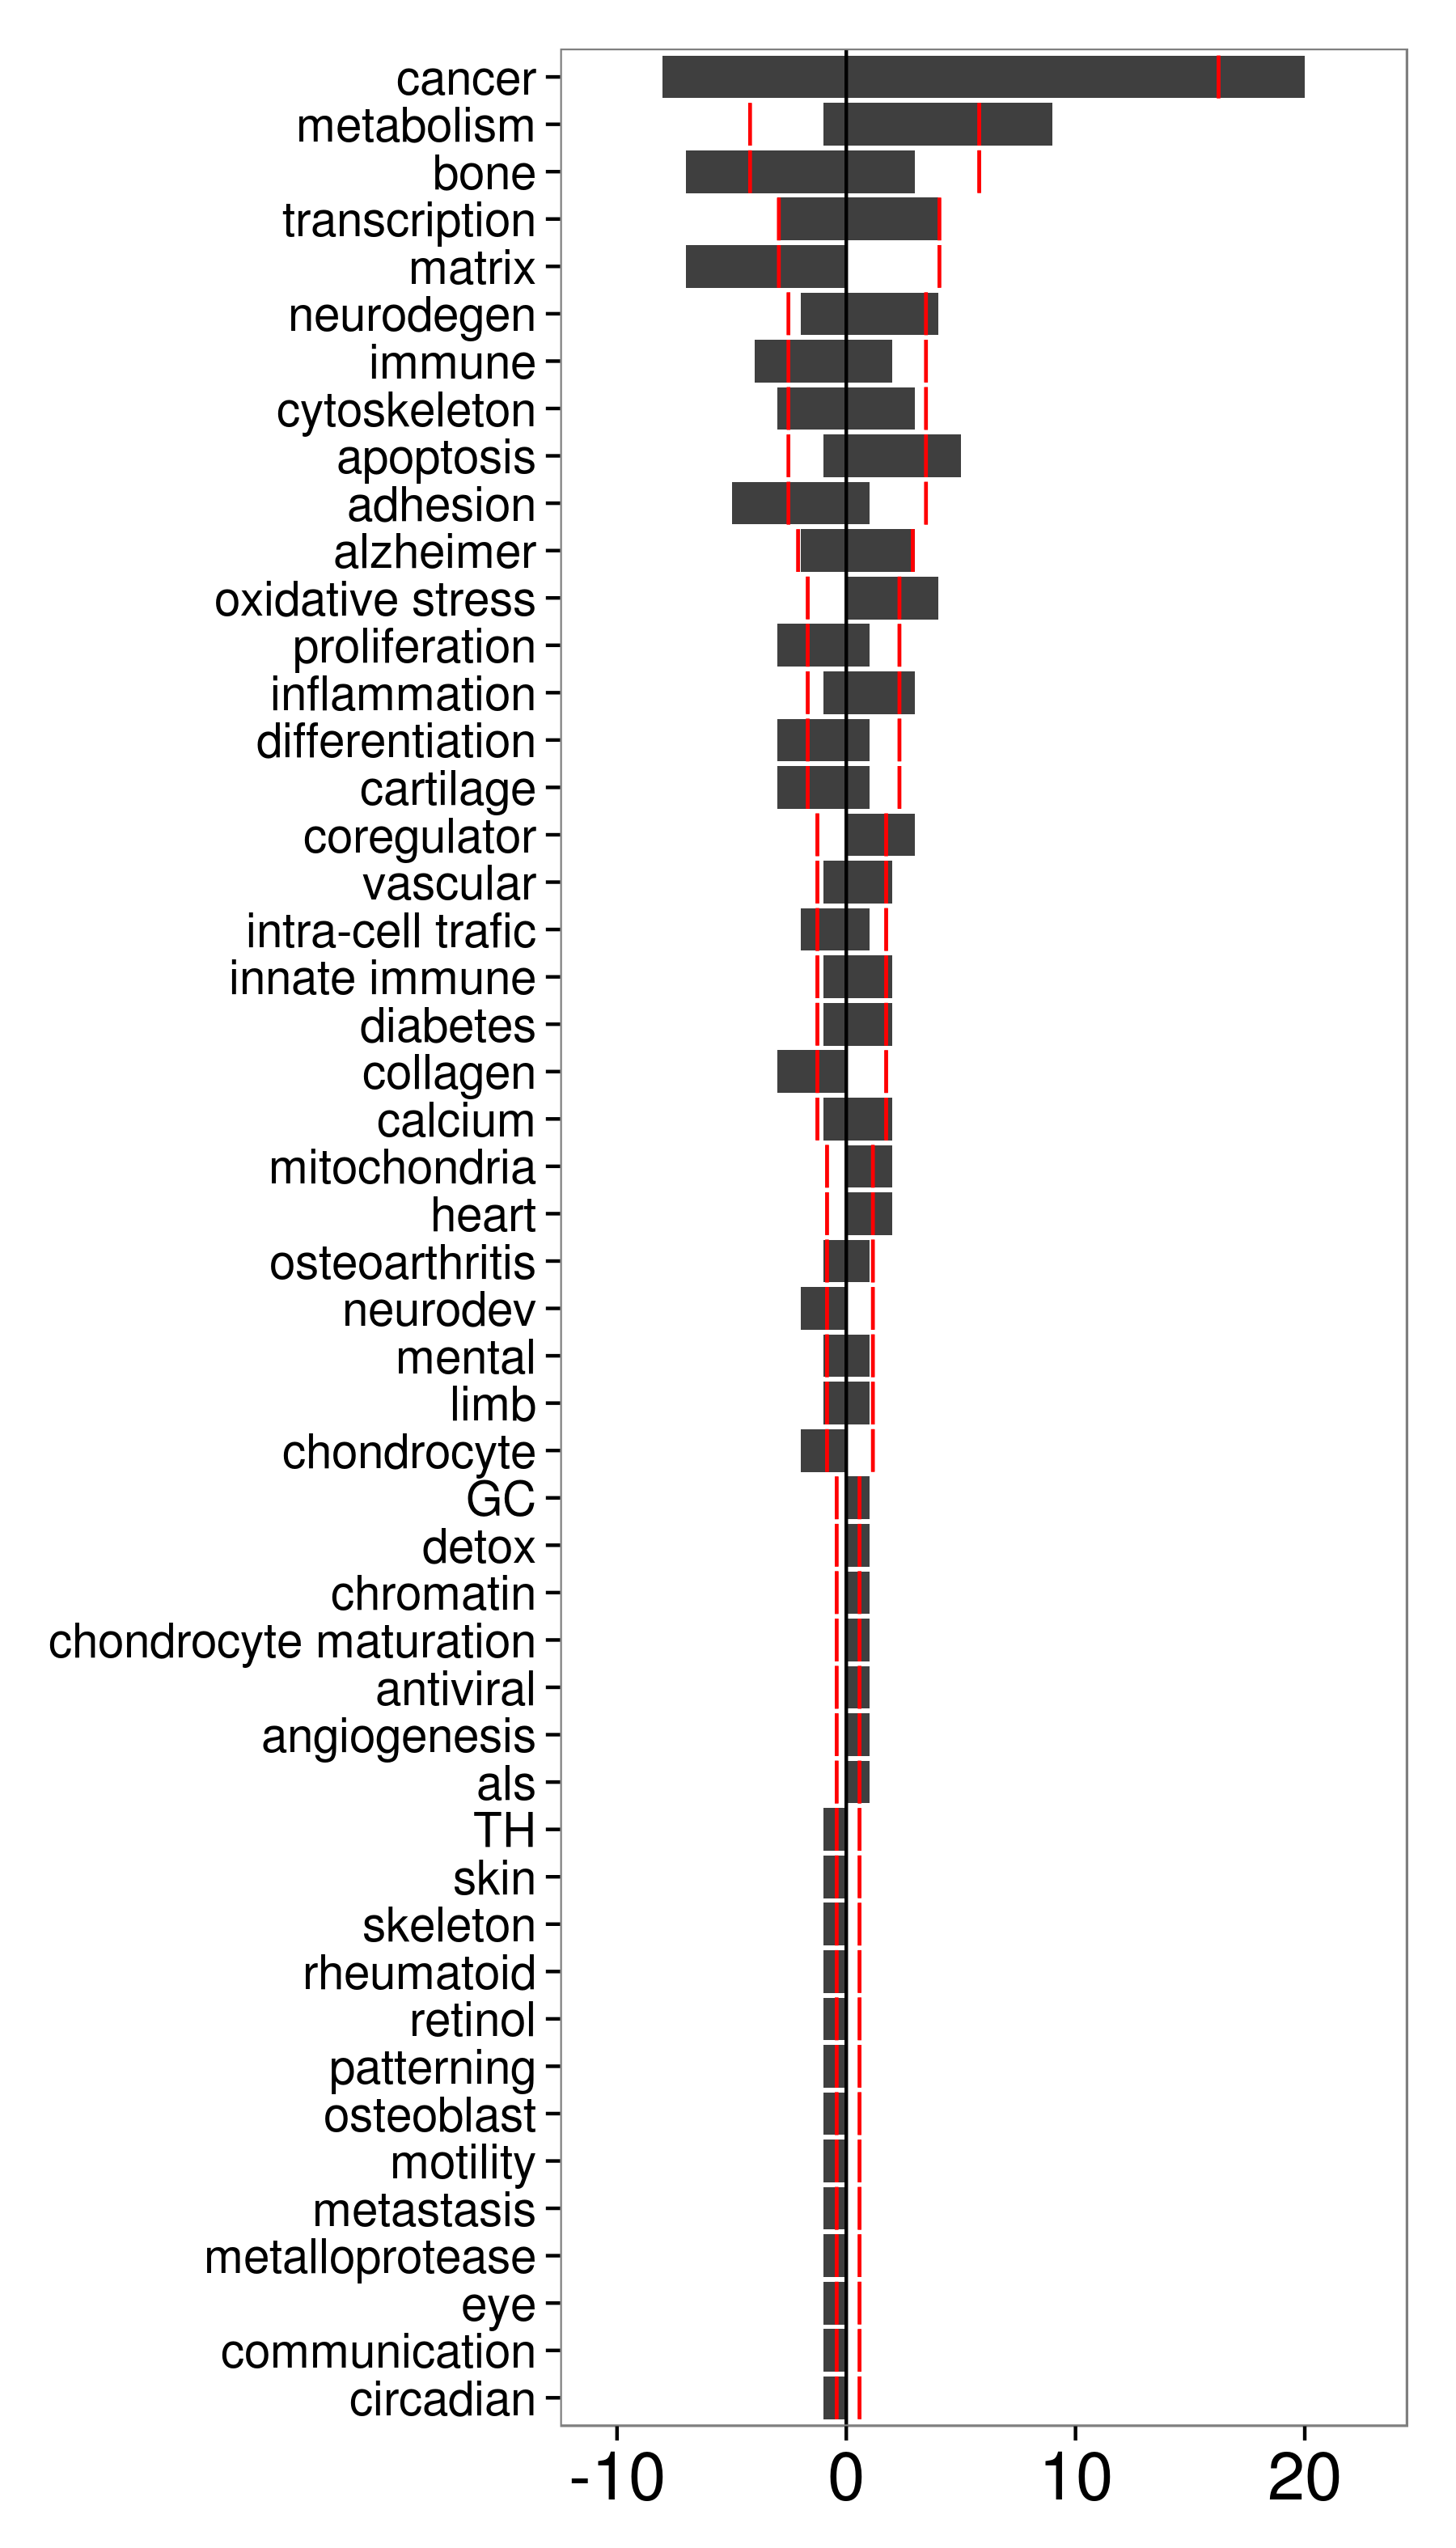
\includegraphics[width=\textwidth]
	{Figures/tfc-manualannot-antago/tfc-manualannot-antago-c.png}
	\caption{}
	\label{subfig:tfc-manualannot-antago-c}
\end{subfigure}
\begin{subfigure}{0.49\textwidth}
	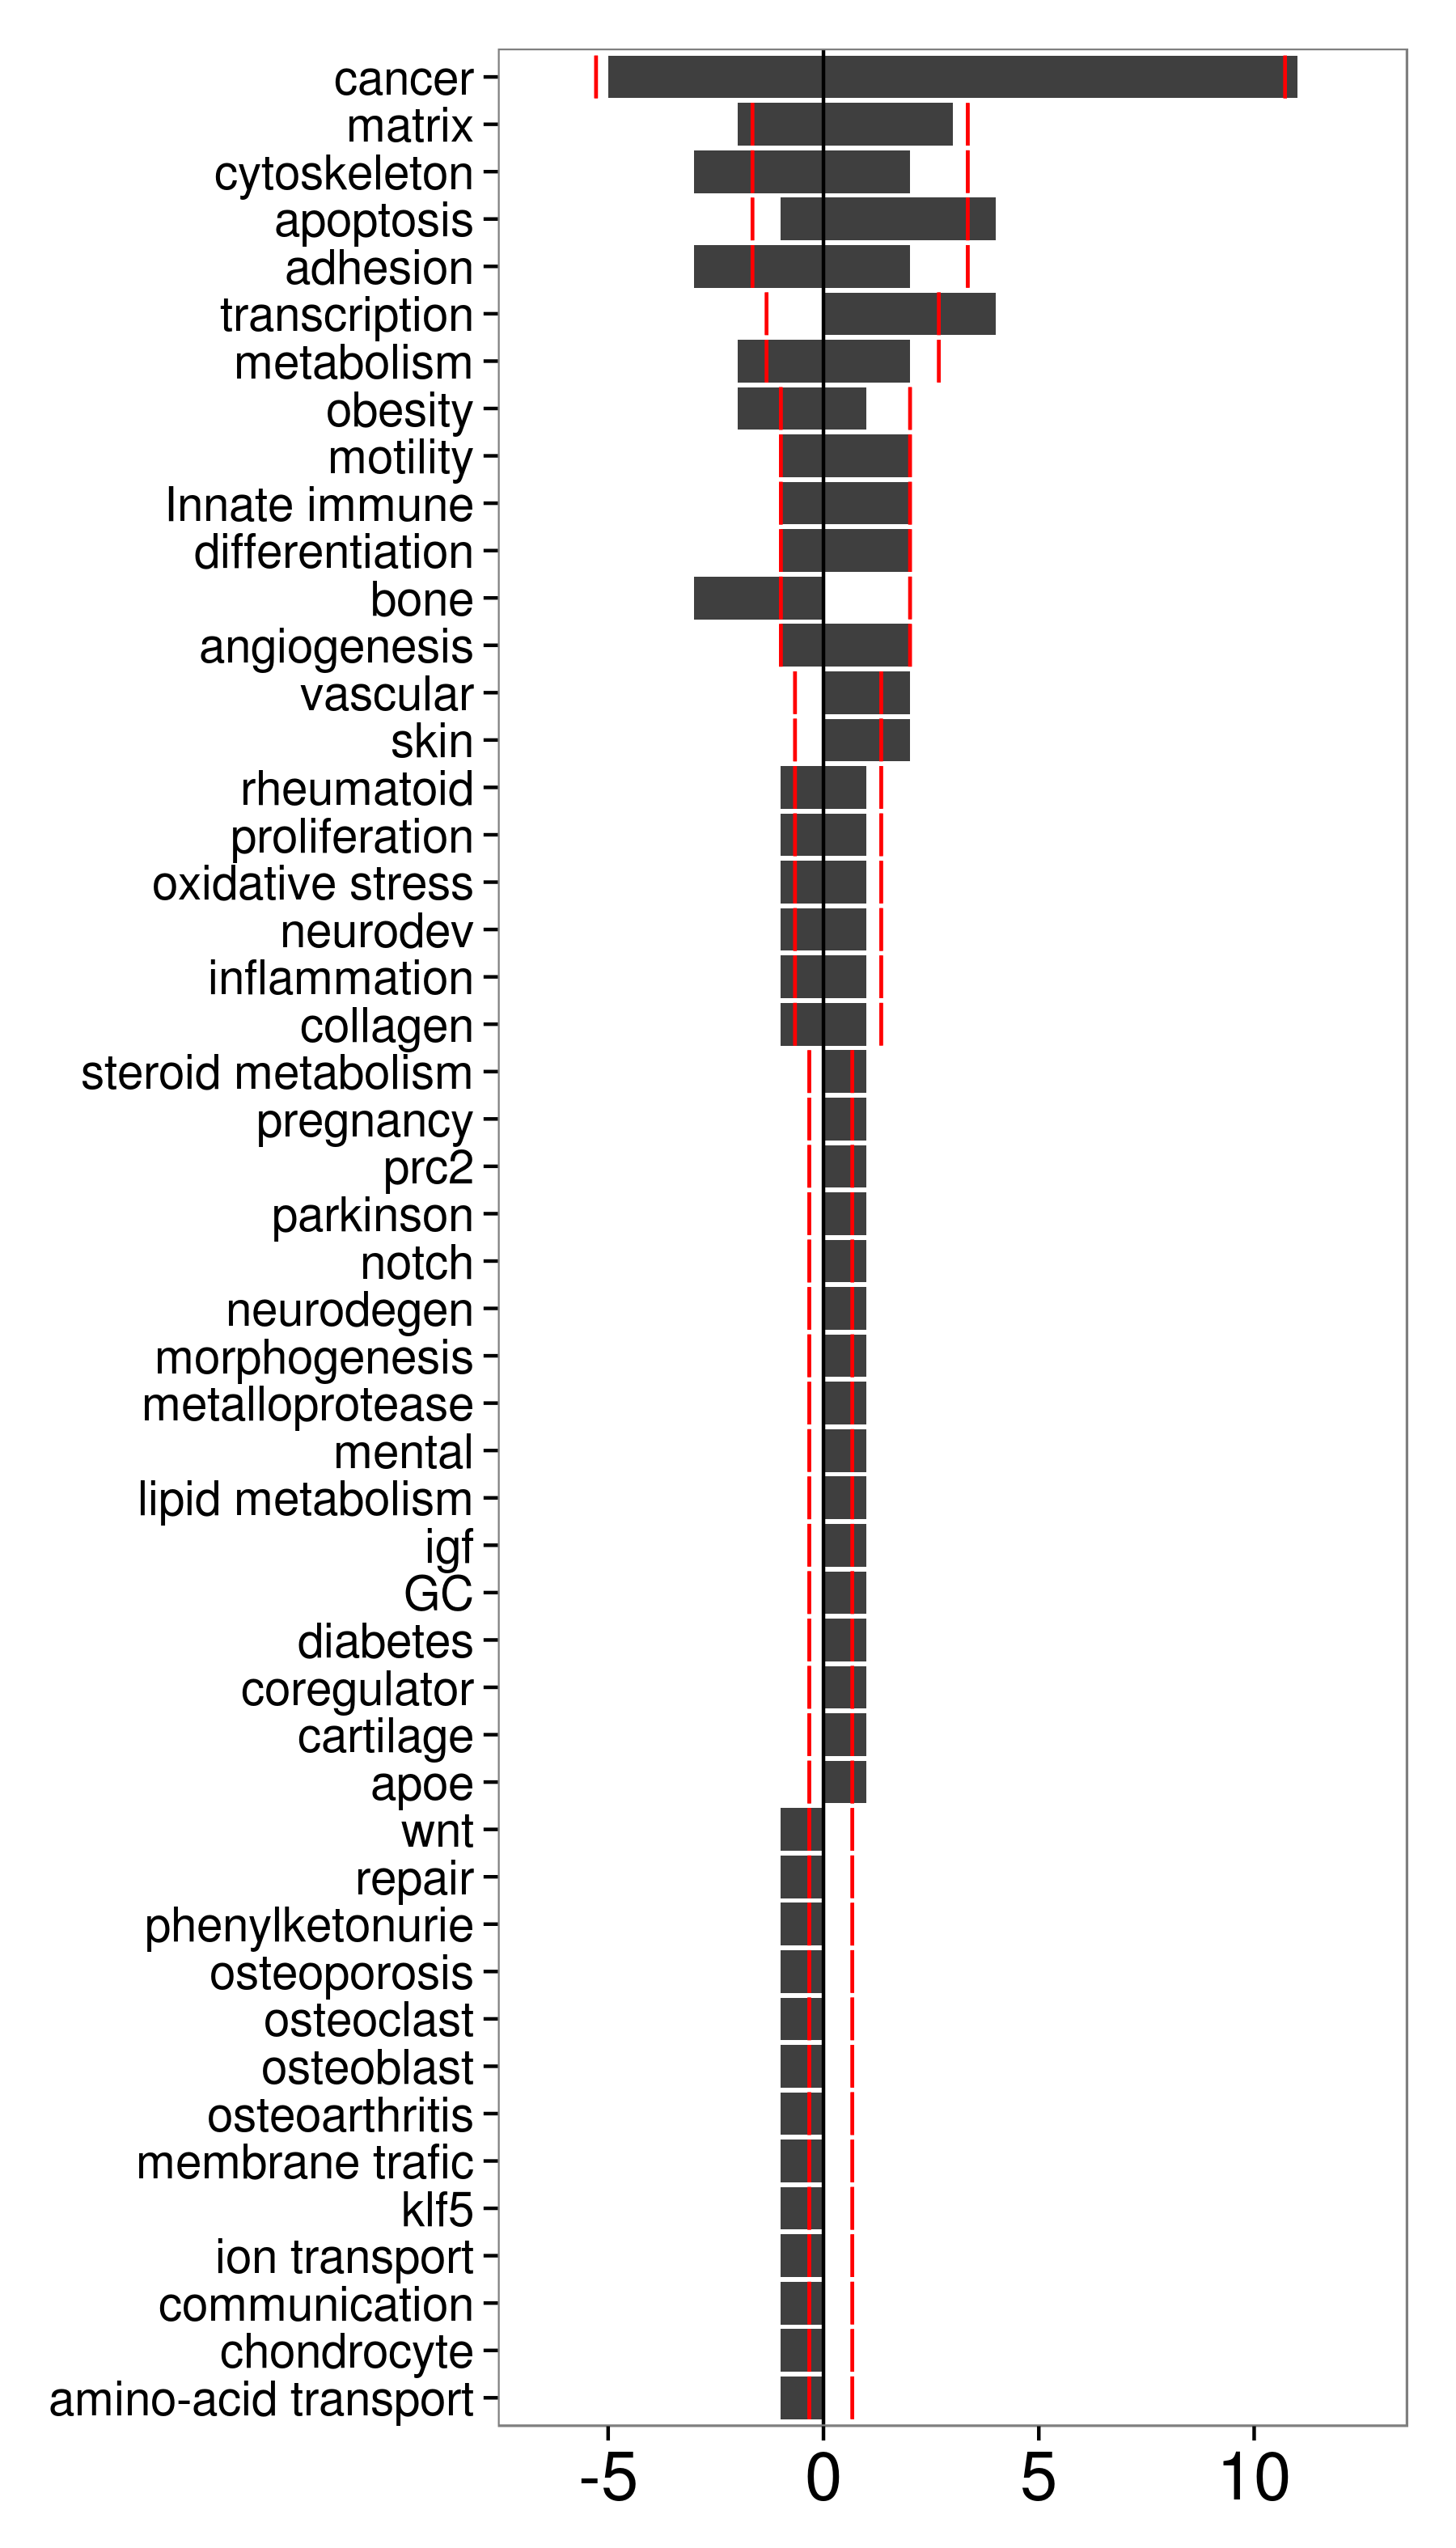
\includegraphics[width=\textwidth]
	{Figures/tfc-manualannot-antago/tfc-manualannot-antago-t.png}
	\caption{}
	\label{subfig:tfc-manualannot-antago-t}
\end{subfigure}
\caption[Catégories fonctionnelles enrichies parmi les gènes ``antagonisés'' dans l'épiderme caudal]
{
Catégories fonctionnelles enrichies parmi les gènes présentant un profil ``d'antagonisation'' et réprimés (valeurs négatives, partie gauche de chaque sous-figure) ou induits (valeurs positives, partie droite de chaque sous-figure) dans l'épiderme caudal.
\ref{subfig:tfc-manualannot-antago-c} Effets de la \gls{cort} antagonisé par la \gls{t3}, correspondant aux clusters 1-4 de la \autoref{fig:tfc-clusters-antago}~A.
\ref{subfig:tfc-manualannot-antago-t} Effets de la \gls{t3} antagonisé par la \gls{cort}, correspondant aux clusters 5-6 de la \autoref{fig:tfc-clusters-antago}~B.
La valeur absolue de l'axe des abscisses représente le nombre de gène associé à chaque terme (axe des ordonnées).
Seuls les 50 termes les plus représenté sont illustrés ici.
Les barres verticales rouge correspondent au nombre théorique de gènes associés à chaque terme dans le cas d'une répartition aléatoire entre répression et induction.
}
\label{fig:tfc-manualannot-antago}
% ===========================================================
%
% BOTTOM caption
% ------------------------
\end{figure}
% ------------------------

De façon frappante, il semble que le termes enrichis soient très spécifiques des tissus, en particulier dans le cas de l'antagonisme de l'effet \gls{t3}
par la \gls{cort}.
Cette dichotomie se traduit par l'enrichissement de termes liés au métabolisme, au devenir cellulaire et au stress oxidatif pour les gènes induits par la \gls{t3}; de termes liés au remodelage de la matrice extra-cellulaire parmi les gènes réprimés.
Le même type de dichotomie est observée pour les gènes dont l'effet de la \gls{cort} est antagonisé par la \gls{t3}, mais dans une moindre mesure.


\subsection{Annotation manuelle des gènes constituant les profils "potentiés"}
Enfin, le même type d'analyse pour les gènes "potentiés" (\autoref{fig:tfc-manualannot-pot}) ne révèle pas de fonction biologique préférentiellement associée au sens de la variation (si ce n'est le métabolisme qui tend à être légèrement enrichi parmi les gènes induits).

% BOTTOM caption
% ------------------------
\begin{figure}[!htbp]
\centering
\vspace{1\baselineskip}
\includegraphics[width=0.9\textwidth]
% ------------------------
%
% SIDE caption
% ------------------------
%\begin{SCfigure}[\sidecaptionrelwidth][!htbp]
%\centering
%\vspace{1\baselineskip}
%\includegraphics[width=0.5\textwidth]
% ------------------------
%
% Main information
% ===========================================================
{Figures/tfc-manualannot-pot/tfc-manualannot-pot.png}
\caption[Termes enrichis dans les catégories de type ``potentiation'' dans l'épiderme caudal]
{
Termes enrichis dans les catégories de type ``potentiation'' entre les effets des deux hormones dans l'épiderme caudal.
Les valeurs négatives (partie gauche) correspondent à une potentiation de l'effet répresseur des hormones.
Les valeurs positives (partie droite) correspondent à une potentiation de l'effet inducteur des hormones.
La valeur absolue de l'axe des abscisses représente le nombre de gènes associé à chaque terme (axe des ordonnées).
Seuls les 50 termes les plus représenté sont illustrés.
Les barres verticales rouges correspondent au nombre théorique de gènes associés à chaque terme dans le cas d'une répartition aléatoire entre répression et induction.
}
\label{fig:tfc-manualannot-pot}
% ===========================================================
%
% BOTTOM caption
% ------------------------
\end{figure}
% ------------------------
%
% SIDE caption
% ------------------------
%\end{SCfigure}
% ------------------------

La majorité des gènes réprimés sont ici associés à des processus apoptotiques et de prolifération, au remodelage de la matrice extra-cellulaire, à l'adhésion et à la réponse du système immunitaire inné.

\end{document}